\section{Proof attempts without Chowla}\label{sec:bypass}

The logarithmic correlation theorem was used for the obstruction in Section~\ref{sec:tao}. The two constructions below use only one-variable Dirichlet series and Mellin transforms. They give different sufficient estimates for RH.

\subsection{A single smooth weight that detects every right-hand zero}

Let \(B(X)=\sum_{n\ge1}\lambda(n)e^{-n/X}\) for \(X>0\). This sum is absolutely convergent. For \(\R s>1\), absolute convergence and the substitution \(y=n/X\) give
\begin{equation}\label{eq:gamma}
 \int_0^\infty B(X)X^{-s}\frac{\dd X}{X}
 =\Gamma(s)\frac{\zeta(2s)}{\zeta(s)}.
\end{equation}
The integral over \(0<X\le1\) is entire because \(|B(X)|\le e^{-1/X}/(1-e^{-1/X})\).

\begin{proposition}[A smoothed bypass]\label{prop:smoothed}
For \(1/2\le\theta\le1\), the bound \(B(X)\ll_{\varepsilon,\theta}X^{\theta+\varepsilon}\) for all \(\varepsilon>0\) is equivalent to the zero-free condition \(\zeta(s)\ne0\) for \(\R s>\theta\).
\end{proposition}
\begin{proof}
Under the bound, the integral in \eqref{eq:gamma} is holomorphic on \(\R s>\theta\). The identity extends meromorphically, and neither \(\Gamma(s)\) nor \(\zeta(2s)\) vanishes there. For the converse use Theorem~\ref{thm:equiv} and the partial summation identity
\(
 B(X)=X^{-1}\int_1^\infty L(u)e^{-u/X}\dd u.
\)
Changing \(u=Xv\) gives the required bound for \(X\ge1\).
\end{proof}

The nonvanishing of the Mellin weight in \eqref{eq:gamma} matters. In the recent work of Li, Sun and Wang \cite{lsw}, a particularly effective weight is built from \(W(x)=\sum_{m\ge1}V(mx)\), where \(V\) is smooth, compactly supported in \((0,\infty)\), and \(\int_0^\infty V=0\). At each \(X>0\) the sums below are finite. Complete multiplicativity gives
\[
 \sum_{n\ge1}\lambda(n)W(n/X)=
 \sum_{r\ge1}V(r/X)\sum_{n\mid r}\lambda(n)
 =\sum_{j\ge1}V(j^2/X).
\]
Indeed \(\sum_{k=0}^\ell (-1)^k\) is \(1\) when \(\ell\) is even and \(0\) otherwise, which proves the divisor identity prime by prime. The sum on the right is \(O_V(\sqrt X)\) for \(X\ge1\), by the support of \(V\). For \(\R s>1\), however, the Mellin transform of \(W\) is \(\zeta(s)\widehat V(s)\), where \(\widehat V(s)=\int_0^\infty V(x)x^{s-1}\dd x\). The equality continues to the right half-plane by Poisson summation. To see the convergence at zero, extend \(V\) by zero to \(\mathbb R\) and write \(\sum_{m\in\mathbb Z}V(mx)=x^{-1}\sum_{k\in\mathbb Z}\widehat V_{\mathrm F}(k/x)\), with \(\widehat V_{\mathrm F}\) the Fourier transform. The \(k=0\) term vanishes and the others decay faster than any fixed power as \(x\downarrow0\). The factor \(\zeta(s)\) cancels the very poles that the Mellin test needs to detect.\footnote{Li, Sun and Wang also construct a different weight adapted to a specified zero in their Appendix A. The pole cancellation here concerns the divisor-convolution weight only.}

\subsection{Reciprocal dilates with an explicit error rate}

The Nyman--Beurling criterion and its discrete strengthening \cite{baez,burnol} suggest working with reciprocal dilates. For \(n\ge1\), define the balanced functions
\[
 g_n(x)=\{1/(nx)\}-n^{-1}\{1/x\},\qquad x>0.
\]
They vanish for \(x>1\). For \(1/2\le\sigma<1\), set
\[
 \|u\|_\sigma^2=\int_0^1 |u(x)|^2 x^{2\sigma-1}\dd x,\qquad
 d_{M,\sigma}=\inf_{c_1,\ldots,c_M\in\mathbb C}
      \left\|1-\sum_{n\le M}c_ng_n\right\|_\sigma.
\]
The norm at \(\sigma=1/2\) is the ordinary \(L^2(0,1)\) norm. The functions \(\{nx\}\) considered in \cite{nbdraft} form a different approximation problem. Appendix~\ref{sec:ordinary} solves that finite problem and explains the difference.

\begin{lemma}[Exact Mellin transform]\label{lem:nbmellin}
For \(0<\R s<1\),
\[
 \int_0^1 g_n(x)x^{s-1}\dd x
 =-(n^{-s}-n^{-1})\frac{\zeta(s)}{s}.
\]
\end{lemma}
\begin{proof}
After substituting \(y=1/(nx)\) in the integral of the unbalanced function over \(x>0\), the transform is \(n^{-s}\int_0^\infty\{y\}y^{-s-1}\dd y\). On \(0<y<1\) the integral is \(1/(1-s)\). On \(y>1\) it is \(1/(s-1)-\zeta(s)/s\) by the Euler summation identity in Appendix~\ref{sec:perron}. The two rational terms cancel. Subtract the corresponding \(n^{-1}\) multiple of the \(n=1\) transform and use the support of \(g_n\).
\end{proof}

\begin{theorem}[Convergence in shifted norms]\label{thm:shifted}
Suppose \(1/2\le\theta<\sigma<1\) and \(\zeta\) has no zero in \(\R s>\theta\). For each \(0<\delta<\sigma-\theta\), the explicit choice
\[
 c_n=-\mu(n)(1-n/M)\qquad (n\le M)
\]
satisfies \(\|1-\sum_{n\le M}c_ng_n\|_\sigma\ll_{\sigma,\theta,\delta}M^{-\delta}\). Conversely, for every nontrivial zero \(\rho\) with \(\R\rho>\sigma\),
\[
 d_{M,\sigma}^2\ge \frac{2(\R\rho-\sigma)}{|\rho|^2}
 \quad\text{for every }M .
\]
\end{theorem}
\begin{proof}
Let \(D_M(s)=\sum_{n\le M}\mu(n)(1-n/M)n^{-s}\). For \(s=\sigma+it\), absolute convergence on \(\R w=2\) gives
\[
 D_M(s)=\frac1{2\pi i}\int_{\R w=2}
        \frac{M^w}{w(w+1)\zeta(s+w)}\dd w .
\]
The scalar kernel identity follows by closing left when \(M/n>1\), with residues \(1\) and \(-n/M\), and closing right when \(M/n<1\). At \(n=M\) the kernel is zero by continuity, using absolute convergence on \(\R w=2\).

Move the contour to \(\R w=-\delta\). There is only the residue \(1/\zeta(s)\) at \(w=0\). There are no poles from zeros because \(\sigma-\delta>\theta\), and \(-\delta>-1\). Lemma~\ref{lem:subpower} and the Euler product to its right show that the horizontal integrals tend to zero for each fixed \(t\). On the new vertical line the integral is
\[
 O_{\sigma,\theta,\delta,\eta}
 \left(M^{-\delta}\int_{\mathbb R}
 \frac{(1+|t+v|)^\eta}{(1+|v|)^2}\dd v\right)
 =O_{\sigma,\theta,\delta,\eta}(M^{-\delta}(1+|t|)^\eta)
\]
for \(0<\eta<1\). The last equality follows from \(1+|t+v|\le(1+|t|)(1+|v|)\). The same argument at \(s=1\) gives \(D_M(1)=O(M^{-\delta})\) because \(1/\zeta(1)=0\) in the removable extension.

By Lemma~\ref{lem:nbmellin}, the residual has Mellin transform \([1-\zeta(s)(D_M(s)-D_M(1))]/s\). The proof of Lemma~\ref{lem:subpower} bounds \(|\zeta(s)|\) by \(O((1+|t|)^\eta)\) on \(\R s=\sigma\) as well, using \(+\R G\) instead of \(-\R G\). Thus the residual transform is \(O(M^{-\delta}(1+|t|)^{2\eta-1})\). For \(\eta<1/4\) its square integrates. Apply Plancherel to \(e^{-\sigma y}u(e^{-y})\one_{y>0}\) with \(y=-\log x\). Its squared norm is \(\|u\|_\sigma^2\), and its Fourier transform in angular frequency is the Mellin transform on \(\R s=\sigma\). This proves the upper bound.

If \(\R\rho>\sigma\), the residual evaluates to \(1/\rho\) at \(\rho\). Cauchy--Schwarz in the weighted space bounds the absolute value of the evaluation by \(\|u\|_\sigma(2(\R\rho-\sigma))^{-1/2}\). This proves the lower bound uniformly in the coefficients.
\end{proof}

Taking the published quasi-Riemann manuscript as input gives convergence for \(\sigma>7/8\). The proof loses its positive choice of \(\delta\) as \(\sigma\downarrow7/8\). For a proof of RH, it would suffice to find any sequence of balanced reciprocal-dilate polynomials for which the residual tends to zero at \(\sigma=1/2\), by the lower bound in Theorem~\ref{thm:shifted} and the functional equation.\footnote{A boundary point on \(\R s=\sigma\) is not a bounded evaluation in the weighted Hilbert space. The argument for a hypothetical zero strictly to the right therefore gives no pointwise evaluation bound on the line itself.} The explicit construction proves the convergence away from the zero-free boundary. It leaves the critical norm unbounded by a quantity tending to zero.

One can quantify the cost of trying to reach the critical norm by interpolation. For \(0<\sigma_0<1/2<\sigma_1<1\), H\"older's inequality gives
\[
 \|u\|_{1/2}\le \|u\|_{\sigma_0}^{1-t}\|u\|_{\sigma_1}^{t},
 \qquad t=\frac{1/2-\sigma_0}{\sigma_1-\sigma_0}.
\]
For the explicit residual \(u_M=1-\sum c_ng_n\), the trivial coefficient bound gives \(\|u_M\|_{\sigma_0}\ll_{\sigma_0}M^{1-\sigma_0}\). Indeed, write \(x=1/y\). For \(n\le y\), \(|g_n(1/y)|\le 2\), and for \(n>y\), \(|g_n(1/y)|=\lfloor y\rfloor/n\). Consequently \(|u_M(1/y)|\ll y(1+\log(M/y))\) when \(1\le y\le M\), and \(|u_M(1/y)|\ll M\) otherwise. Integrating the square with weight \(y^{-2\sigma_0-1}\) gives the stated bound, using \(y=Mv\) in the first integral. Even with \(\delta\) at its limiting value \(\sigma_1-\theta\), the numerator of the interpolated exponent is
\[
 (\sigma_1-\tfrac12)(1-\sigma_0)
  -(\tfrac12-\sigma_0)(\sigma_1-\theta)
 =\tfrac12(\sigma_1-\tfrac12)+(\tfrac12-\sigma_0)(\theta-\tfrac12)>0 .
\]
Thus this interpolation with the available lower-norm estimate cannot prove decay at \(1/2\).

\begin{figure}[ht]
\centering
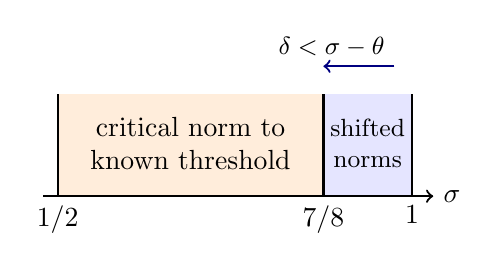
\begin{tikzpicture}[x=9cm,y=1cm]
\fill[orange!14] (.5,0) rectangle (.875,1.3);
\fill[blue!10] (.875,0) rectangle (1,1.3);
\draw[->,thick] (.48,0)--(1.03,0) node[right] {\(\sigma\)};
\foreach \x/\t in {.5/{1/2},.875/{7/8},1/{1}} {
 \draw[thick] (\x,0)--(\x,1.3);
 \node[below] at (\x,0) {\(\t\)};
}
\node[align=center] at (.6875,.67) {critical norm to\\known threshold};
\node[align=center,font=\small] at (.9375,.67) {shifted\\norms};
\draw[->,thick,blue!50!black] (.975,1.65)--(.875,1.65);
\node[anchor=south east,font=\small] at (.975,1.65) {\(\delta<\sigma-\theta\)};
\end{tikzpicture}
\caption{The shifted-norm construction with the \(7/8\) input. The rate in Theorem~\ref{thm:shifted} depends on the distance to the right of the zero-free boundary.}
\label{fig:strip}
\end{figure}

\subsection{Why the explicit family stops at the critical norm}

The failed interpolation does not settle whether the same coefficients might converge by a different argument. The following rescaling calculation answers that question. The obstruction is present even if all zeta zeros lie on the line. For related failures of natural approximants, see B\'aez-Duarte \cite{bd-arith}.

\begin{theorem}[A critical-norm obstruction for the linear Riesz family]\label{thm:riesz-failure}
For \(M\ge2\) let
\[
 u_M(x)=1+\sum_{n\le M}\mu(n)(1-n/M)g_n(x).
\]
Then \(\limsup_{M\to\infty}\|u_M\|_{1/2}>0\). The infimum over coefficients defining \(d_{M,1/2}\) is a separate problem.
\end{theorem}
\begin{proof}
Put \(b_m=\sum_{n\mid m}n\mu(n)=\prod_{p\mid m}(1-p)\) and \(B_1(y)=\sum_{m\le y}b_m\). For \(1\le y\le M\),
\begin{equation}\label{eq:riesz-rescale}
 u_M(1/y)=\lfloor y\rfloor D_M(1)+M^{-1}B_1(y).
\end{equation}
Indeed \(g_n(1/y)=\lfloor y\rfloor/n-\lfloor y/n\rfloor\). In the second term the unweighted sum \(\sum_{n\le M}\mu(n)\lfloor y/n\rfloor\) equals \(1\), by the divisor identity \(\sum_{n\mid m}\mu(n)=\one_{m=1}\). The remaining weighted sum is \(B_1(y)/M\). Formula \eqref{eq:riesz-rescale} holds for real \(M\) as well as integers.

Suppose that \(\|u_M\|_{1/2}\to0\) along the integers. The same would hold for real \(M\). To see this, put \(m=\lfloor M\rfloor\). Only the coefficients at \(n\le m\) contribute to the difference, and their differences have absolute value at most \(n/m^2\). As \(|g_n|\le2\), the differences of the functions are uniformly bounded. At fixed \(x=1/y\in(0,1)\), for \(n>y\) one has \(g_n(x)=\lfloor y\rfloor/n\), so the difference tends to zero pointwise. Dominated convergence gives the claim.

Choose a nontrivial zero \(\rho=1/2+i\gamma\) on the line, whose existence is classical, and put \(s_0=1+\rho\). Choose \(W\in C_c^\infty(0,1)\) with
\[
 \int_0^1 vW(v)\dd v=0,\qquad
 \int_0^1 v^{s_0}W(v)\dd v\ne0.
\]
Such a weight can be constructed from a nonnegative bump \(\psi\) supported on a closed interval \([a,b]\subset(0,1)\). Set \(W=\psi(\overline{v^{s_0}}-c v)\) with \(c=\int\psi v\,\overline{v^{s_0}}/\int\psi v^2\). Strict Cauchy--Schwarz gives the second condition because \(v^{s_0}\) is not proportional to \(v\) on an open interval.

Write \(G(X)=\int_0^1 B_1(Xv)W(v)\dd v\). Applying \eqref{eq:riesz-rescale} on the support of \(W\) for \(X\ge1/a\) gives
\[
 X^{-3/2}G(X)=X^{-1/2}\int_0^1 u_X(1/(Xv))W(v)\dd v
 +O_W\bigl(X^{-1/2}|D_X(1)|\bigr).
\]
The vanishing moment eliminates \(Xv\) from the floor term. Since \(|D_X(1)|\ll\log(2X)\), the error tends to zero. In the main term, substitute \(x=1/(Xv)\) and apply Cauchy--Schwarz. This bounds its absolute value by
\[
 \|vW\|_{L^2(0,1)}\|u_X\|_{1/2}.
\]
Thus \(G(X)=o(X^{3/2})\) would follow.

For \(\R s>2\), absolute convergence and partial summation give
\[
 \int_0^\infty G(X)X^{-s-1}\dd X
 =\left(\int_0^1 v^s W(v)\dd v\right)
   \frac{\zeta(s)}{s\,\zeta(s-1)} .
\]
In detail, the Mellin integral of \(B_1\) is \(s^{-1}\sum b_m m^{-s}\). Its Dirichlet series is \(\zeta(s)/\zeta(s-1)\) by the divisor formula for \(b_m\). Substitution \(y=Xv\) gives the factor in parentheses. The assumed little-oh bound makes the left side holomorphic on \(\R s>3/2\). It also implies that its value at \(s_0+\epsilon\), multiplied by \(\epsilon\), tends to zero as \(\epsilon\downarrow0\). Split the integral at a fixed large \(X_0\) and bound the tail using \(|G(X)|\le o_{X_0\to\infty}(1)X^{3/2}\) for \(X\ge X_0\).

The right side has a pole at \(s_0\) by the choice of \(W\), the Euler product at \(\R s_0=3/2\), and the zero of \(\zeta(s_0-1)\). The meromorphic identity theorem gives a contradiction to the last limit, regardless of the multiplicity of \(\rho\). This excludes the assumed convergence.
\end{proof}

For a simple \(\rho\), the same calculation gives the lower bound
\[
 \limsup_M\|u_M\|_{1/2}\ge
 \frac{|\zeta(s_0)\int_0^1 v^{s_0}W(v)\dd v|}
 {|s_0\zeta'(\rho)|\,\|vW\|_{L^2(0,1)}} .
\]
Indeed, finite limit superior of the norms bounds the limit superior of \(|G(X)|X^{-3/2}\) by that of the norms times \(\|vW\|_2\). The Abel integral bounds the absolute residue by the same quantity. If \(\rho\) is multiple, finite limit superior would give only an \(O(\epsilon^{-1})\) bound at \(s_0+\epsilon\), incompatible with its higher-order pole.

\begin{theorem}[Every fixed taper of bounded variation]\label{thm:holder}
Let \(w:[0,1]\to\mathbb C\) have bounded variation and \(w(0+)=1\). Define
\[
 U_M(x)=1+\sum_{n\le M}\mu(n)w(n/M)g_n(x).
\]
For each nontrivial zero \(\rho\) with \(\beta=\R\rho\ge1/2\),
\[
 \limsup_{M\to\infty} M^{1/2-\beta}\|U_M\|_{1/2}>0.
\]
This limit superior is infinite if \(\rho\) is multiple. In particular the residuals cannot converge to zero in the critical norm, even under RH. The result includes every fixed real order \(r>0\) of Riesz smoothing, \(w(t)=(1-t)^r\).
\end{theorem}
\begin{proof}
Extend \(w\) by zero on \(t>1\), and set \(f(t)=1-w(t)\) for \(t>0\). Thus \(f\) is bounded, with limits zero at zero and one at infinity. For \(X\ge2\) real let \(D_{X,w}(1)=\sum_{n\le X}\mu(n)w(n/X)/n\). The divisor identity used in \eqref{eq:riesz-rescale} now gives, for \(Xv\ge1\),
\begin{equation}\label{eq:general-rescale}
 U_X(1/(Xv))=\lfloor Xv\rfloor D_{X,w}(1)
       +\sum_{n\le Xv}\mu(n)f(n/X)\lfloor Xv/n\rfloor .
\end{equation}
There is no restriction \(v\le1\) here, since \(w\) has been extended by zero.

Passing from integer \(m=\lfloor X\rfloor\) to real \(X\) changes the residual by \(o(1)\) in the critical norm. Indeed \(n/X\in[(n-1)/m,n/m]\) for \(n\le m\), so \(\sum_{n\le m}|w(n/X)-w(n/m)|\) is at most the total variation of \(w\). The residual difference is uniformly bounded by \(2\operatorname{Var}(w)\). At fixed \(y\ge1\), the finitely many terms \(n\le K\) tend to zero as \(m\to\infty\). For \(K>y\), the remaining terms contribute at most \(\lfloor y\rfloor\operatorname{Var}(w)/K\), because \(g_n(1/y)=\lfloor y\rfloor/n\) for \(n>y\). Let \(K\to\infty\) and use dominated convergence. The passage to real \(X\) preserves the scaled limit superior for \(\beta\ge1/2\).

Take a test function \(W\in C_c^\infty(0,\infty)\) with \(\int vW(v)\dd v=0\) and write
\[
 K_W(t)=f(t)\int_0^\infty W(v)\lfloor v/t\rfloor\dd v .
\]
The integral factor equals \(-\int W(v)\{v/t\}\dd v\) by the first moment condition. It is bounded at zero and vanishes for \(t>\sup\operatorname{supp} W\). Therefore \(\widehat K_W(s)=\int_0^\infty K_W(t)t^{s-1}\dd t\) is holomorphic on \(\R s>0\). With \(H(X)=\sum_{n\ge1}\mu(n)K_W(n/X)\), equation \eqref{eq:general-rescale} and the rescaling of the norm give
\[
 |H(X)|\ll_W \sqrt X\,\|U_X\|_{1/2}+\log(2X)
\]
for large \(X\). The logarithmic term comes from replacing \(\lfloor Xv\rfloor\) by \(Xv\) and using \(D_{X,w}(1)=O(\log(2X))\). For \(\R s>1\), termwise integration gives
\begin{equation}\label{eq:general-inverse}
 \int_0^\infty H(X)X^{-s-1}\dd X=\frac{\widehat K_W(s)}{\zeta(s)} .
\end{equation}

We show that \(W\) can be chosen with \(\widehat K_W(\rho)\ne0\). By Fubini,
\[
 \widehat K_W(\rho)=\int_0^\infty W(v)J_\rho(v)\dd v,\qquad
 J_\rho(v)=-\int_0^\infty f(t)\{v/t\}t^{\rho-1}\dd t .
\]
The integral is absolutely convergent because \(0<\beta<1\), and the substitution \(t=v/u\) bounds \(|J_\rho(v)|\ll v^\beta\). It is continuous by dominated convergence on compact \(v\)-intervals, since for fixed \(v\) only a null set of \(t\) lies at jumps of \(\{v/t\}\). If every test of first moment zero annihilated it, it would be proportional to \(v\) as a distribution and hence as a continuous function. For instance, subtract a multiple of a fixed smooth test of first moment one from an arbitrary test. The growth bound at infinity then forces \(J_\rho\equiv0\).

To see why this is impossible, put \(F(r)=f(e^r)\) and \(k_\rho(u)=\{e^u\}e^{-\rho u}\) for \(r,u\in\mathbb R\). Substitution gives \(e^{-\rho r}J_\rho(e^r)=-(k_\rho*F)(r)\). The kernel \(k_\rho\) is integrable, with exponential tails. Its Fourier transform with convention \(e^{-i\xi u}\) is \(-\zeta(\rho+i\xi)/(\rho+i\xi)\), by the fractional-part integral proved in Lemma~\ref{lem:nbmellin}. Its real zeros are isolated. The distributional derivative \(\nu=\dd F\) is a finite complex measure, since \(F\) has bounded variation. Its total mass is \(F(+\infty)-F(-\infty)=1\). If \(k_\rho*F=0\), differentiation gives \(k_\rho*\nu=0\).\footnote{One may differentiate after pairing with a compactly supported smooth test. Fubini is justified by \(k_\rho\in L^1\), boundedness of \(F\), and finiteness of the variation measure. The convolution \(k_\rho*\nu\) is in \(L^1\).} Fourier transformation gives \(\widehat k_\rho\,\widehat\nu=0\). But \(\widehat\nu\) is continuous and equals \(1\) at zero, so it is nonzero on a neighborhood of zero. This would force \(\widehat k_\rho\) to vanish on that neighborhood, a contradiction. Thus a detecting test exists.

With that choice of \(W\), the right side of \eqref{eq:general-inverse} has a pole at \(\rho\). If the scaled limit superior were zero, then \(H(X)=o(X^\beta)\). The Mellin integral would extend holomorphically to \(\R s>\beta\), and multiplication by \(\epsilon\) at \(\rho+\epsilon\) would give a limit of zero by the Abel estimate in Theorem~\ref{thm:riesz-failure}. This contradicts the pole. If the scaled limit superior were finite, the same argument with \(H(X)=O(X^\beta)\) would give at most \(O(\epsilon^{-1})\) at \(\rho+\epsilon\), which excludes a higher-order pole.
\end{proof}

\begin{corollary}[Exact growth of the linear residual]\label{cor:riesz-growth}
For the linear Riesz family of Theorem~\ref{thm:riesz-failure},
\[
 \limsup_{M\to\infty}
   \frac{\log(1+\|u_M\|_{1/2})}{\log M}=\Theta-\tfrac12,
\]
where \(\Theta\) is as in Corollary~\ref{cor:exponent}. Consequently RH is equivalent to \(\|u_M\|_{1/2}\ll_\varepsilon M^\varepsilon\) for every \(\varepsilon>0\), although these norms do not tend to zero.
\end{corollary}
\begin{proof}
Theorem~\ref{thm:holder} gives the lower bound by taking zeros with real part approaching \(\Theta\). For \(\Theta=1/2\) the lower bound is automatic. For the upper bound take \(s=1/2+it\) in the Riesz formula for \(D_M(s)\) and shift the line of \(w\) to \(\R w=\Theta-1/2+\delta>0\), with \(0<\delta<1/4\). There is no residue. On that line the reciprocal has the bound of Lemma~\ref{lem:subpower} when \(\Theta<1\), or the absolutely convergent Euler bound if \(\Theta=1\). The kernel estimate used in Theorem~\ref{thm:shifted} gives
\[
 |D_M(1/2+it)|\ll_{\delta,\eta}
        M^{\Theta-1/2+\delta}(1+|t|)^\eta .
\]
Also \(|D_M(1)|\ll\log(2M)\). The classical convexity bound \(|\zeta(1/2+it)|\ll_\eta (1+|t|)^{1/4+\eta}\) \cite[Ch.~V]{titchmarsh} makes the Mellin residual
\([1-\zeta(s)(D_M(s)-D_M(1))]/s\)
square integrable with \(L^2\) norm \(O_{\delta,\eta}(M^{\Theta-1/2+\delta})\), using \(\eta<1/8\). Plancherel yields the same bound in the critical norm. Let \(\delta\downarrow0\).
\end{proof}

The obstruction applies to a profile held fixed as \(M\) changes. It leaves the unrestricted finite-dimensional projection problem open. The logarithmic taper of Bettin, Conrey and Farmer \cite{bcf} changes with \(M\) and lies outside the theorem. Its conditional asymptotic uses RH and additional information about reciprocal zeta derivatives.

\subsection{A coefficient cost for adaptive approximants}

The fixed-profile obstruction leaves open coefficients that change shape with \(M\). The following necessary condition applies to every finite choice of coefficients and does not depend on a choice of profile.

\begin{theorem}[Harmonic coefficient cost]\label{thm:adaptive}
Let \(U=1+\sum_{n=2}^M a_ng_n\), let \(d=\|U\|_{1/2}\), and put \(a_n=0\) for \(n>M\). For every integer \(K\ge2\),
\[
 \left(\sum_{n\ge2}\frac{|a_n|^2}{n}\right)^{1/2}
 \ge
 \left(\left(\sum_{2\le n\le K}\frac{\mu(n)^2}{n}\right)^{1/2}
            -2d\sqrt K\sum_{m\le K}\frac1m\right)_+ .
\]
Consequently, along any family of approximants with \(d\downarrow0\),
\[
 \sum_{n\ge2}\frac{|a_n|^2}{n}
 \ge\left(\frac{12}{\pi^2}-o(1)\right)\log(1/d).
\]
\end{theorem}
\begin{proof}
The coefficientwise necessity has a precedent in B\'aez-Duarte \cite[Lemma~4.2]{bd-arith}. We give the quantitative estimate. The function \(U(1/y)\) is constant on \(k\le y<k+1\), \(k\ge1\). Write this value as \(V_k\), and define \(V_0=0\). With \(C=\sum_{n\ge2}a_n/n\), the floor formula gives
\[
 V_k=1+kC-\sum_{n\ge2}a_n\lfloor k/n\rfloor,\qquad
 \Delta V_r=C+\one_{r=1}-\sum_{\substack{n\mid r\\n\ge2}}a_n.
\]
M\"obius inversion therefore yields
\(a_n-\mu(n)=-\sum_{r\mid n}\mu(n/r)\Delta V_r\) for every \(n\ge2\).
Also \(d^2=\sum_{k\ge1}|V_k|^2/[k(k+1)]\). Thus
\[
 \sum_{r\le R}\frac{|\Delta V_r|^2}{r}
 \le 2\sum_{r\le R}\frac{|V_r|^2}{r}
       +2\sum_{r\le R}\frac{|V_{r-1}|^2}{r}
 \le4R d^2 .
\]
The first sum is at most \(2(R+1)d^2\), and the second at most \(2(R-1)d^2\), using \(V_0=0\). Minkowski's inequality applied to the divisor sum, with \(n=mr\), now gives
\begin{align*}
 \left(\sum_{2\le n\le K}\frac{|a_n-\mu(n)|^2}{n}\right)^{1/2}
 &\le\sum_{m\le K}\frac1{\sqrt m}
       \left(\sum_{r\le K/m}\frac{|\Delta V_r|^2}{r}\right)^{1/2}
 \\&\le2d\sqrt K\sum_{m\le K}\frac1m .
\end{align*}
The triangle inequality proves the finite bound.

For completeness,
\(\sum_{n\le K}\mu(n)^2/n=(6/\pi^2)\log K+O(1)\).
Indeed \(\mu(n)^2=\sum_{r^2\mid n}\mu(r)\) gives a sum of
\(\mu(r)r^{-2}H_{\lfloor K/r^2\rfloor}\) for \(r\le\sqrt K\). Insert \(H_\ell=\log\ell+\gamma+O(1/\ell)\). The series \(\sum\mu(r)/r^2=1/\zeta(2)\) and \(\sum\mu(r)\log r/r^2\) converge absolutely, and the tail and floor errors are \(O((1+\log K)/\sqrt K)\). Euler's evaluation \(\zeta(2)=\pi^2/6\) gives the coefficient. Finally take \(K=\lfloor d^{-2}/(\log(1/d))^4\rfloor\). The error in the finite bound is \(O(1/\log(1/d))\), while \(\log K=2\log(1/d)+O(\log\log(1/d))\). Squaring proves the claim.
\end{proof}

A uniformly bounded harmonic coefficient norm therefore excludes convergence even for adaptive coefficients. This is a necessary constraint on a possible construction. It gives no lower bound for the unrestricted distance by itself.

\begin{corollary}[Explicit coefficient bound]\label{cor:adaptive-explicit}
For \(0<d\le e^{-4}\), the coefficients in Theorem~\ref{thm:adaptive} satisfy
\[
 \sum_{n\ge2}\frac{|a_n|^2}{n}
 \ge\frac{12}{\pi^2}\log(1/d)
     -\frac{24}{\pi^2}\log\log(1/d)-15 .
\]
\end{corollary}
\begin{proof}
Write \(c=6/\pi^2\). The squarefree identity gives
\(\left|\sum_{n\le t}\mu(n)^2-ct\right|\le3\sqrt t\) for \(t\ge1\), by bounding the floor errors by \(\sqrt t\) and the tail of \(\sum r^{-2}\) by \(2/\sqrt t\). Partial summation then gives \(\sum_{2\le n\le K}\mu(n)^2/n\ge c\log K-7\). Put \(L=\log(1/d)\ge4\) and \(K=\lfloor e^{2L}/L^4\rfloor\). Then \(\log K\ge2L-4\log L-\log2\), and \(2d\sqrt K H_K\le(4L+2)/L^2\le4.5/L\). Apply the finite bound with \(A=(c\log K-7)_+\), use \((\sqrt A-e)_+^2\ge A-2\sqrt A\,e\) and \(\sqrt A\le\sqrt{2cL}\). The cross term is at most \(9\sqrt{2c}/\sqrt L<6.4\), and \(7+c\log2<8\). These bounds give the stated constant \(15\).
\end{proof}

\subsection{A scale-dependent logarithmic taper}

A logarithmic taper is one way to leave the class in Theorem~\ref{thm:holder}. For \(M>1\) set
\begin{align*}
 D_M^{\log}(s)&=\sum_{n\le M}\mu(n)
        \left(1-\frac{\log n}{\log M}\right)n^{-s},\\
 u_M^{\log}&=1+\sum_{n\le M}\mu(n)
        \left(1-\frac{\log n}{\log M}\right)g_n .
\end{align*}
Suppose again that \(\zeta\) has no zeros on \(\R s>\theta\), and fix \(\theta<\sigma<1\). Then \((\log M)u_M^{\log}\) converges in the norm \(\|\cdot\|_\sigma\) to the function with Mellin transform
\begin{equation}\label{eq:logprofile}
 \frac{\zeta(s)+\zeta'(s)/\zeta(s)}{s}\qquad (\R s=\sigma).
\end{equation}
The norm error is \(O(M^{-\delta})\) for every \(0<\delta<\sigma-\theta\). The limit function is \(\lfloor1/x\rfloor-\psi(1/x)\), where \(\psi(y)=\sum_{n\le y}\Lambda(n)\).

\begin{figure}[ht]
\centering
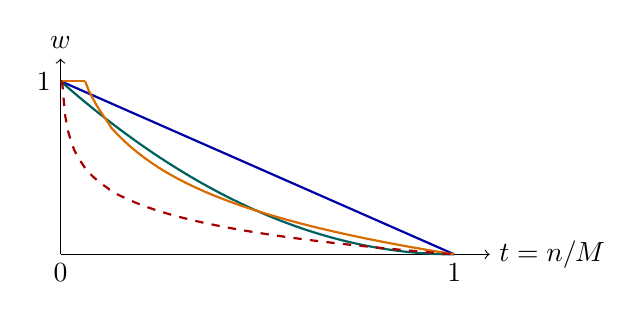
\begin{tikzpicture}[x=5cm,y=2.2cm]
\draw[->] (0,0)--(1.09,0) node[right] {\(t=n/M\)};
\draw[->] (0,0)--(0,1.13) node[above] {\(w\)};
\draw[thick,blue!65!black] (0,1)--(1,0);
\draw[thick,teal!75!black,domain=0:1,samples=60] plot (\x,{(1-\x)^2});
\draw[thick,orange!85!black] (0,1)--(.0625,1);
\draw[thick,orange!85!black,domain=.0625:1,samples=100] plot (\x,{-ln(\x)/ln(16)});
\draw[dashed,thick,red!65!black] (0,1)--(.00390625,1);
\draw[dashed,thick,red!65!black,domain=.00390625:1,samples=130] plot (\x,{-ln(\x)/ln(256)});
\node[below] at (0,0) {\(0\)};
\node[below] at (1,0) {\(1\)};
\node[left] at (0,1) {\(1\)};
\end{tikzpicture}
\par\smallskip
{\small
\textcolor{blue!65!black}{\(1-t\)}\quad
\textcolor{teal!75!black}{\((1-t)^2\)}\quad
\textcolor{orange!85!black}{logarithmic, \(M=16\)}\quad
\textcolor{red!65!black}{logarithmic, \(M=256\)}}
\caption{Fixed profiles and the changing logarithmic profile. The latter is drawn as \(\min(1,-\log t/\log M)\), which agrees with the coefficient taper on \(1/M\le t\le1\). For each fixed \(t>0\) it tends to zero as \(M\) grows.}
\label{fig:tapers}
\end{figure}

To prove this, replace the Riesz kernel by \(M^w/(w^2\log M)\). The scalar inverse transform is \((\log(M/n))_+/\log M\), by the double residue at zero. Shift the line to \(\R w=-\delta\) as in Theorem~\ref{thm:shifted}. For \(F=1/\zeta\) this gives
\[
 D_M^{\log}(s)=F(s)+\frac{F'(s)}{\log M}
       +O_{\sigma,\delta,\eta}\!\left(
          \frac{M^{-\delta}(1+|t|)^\eta}{\log M}\right)
\]
on \(\R s=\sigma\). At \(s=1\), the same calculation gives \(D_M^{\log}(1)=1/\log M+O(M^{-\delta}/\log M)\) since \(F(1)=0\) and \(F'(1)=1\). Insert these formulas in \([1-\zeta(s)(D_M^{\log}(s)-D_M^{\log}(1))]/s\). The leading transform after multiplication by \(\log M\) is \eqref{eq:logprofile}. Lemma~\ref{lem:subpower}, Cauchy's estimate for \(F'\) on a fixed substrip, and the corresponding subpower bound for \(\zeta(s)\) give square integrability. Plancherel bounds the error by \(O(M^{-\delta})\).

For \(1\le y<M\) the formula in the \(x\)-variable is exact:
\[
 (\log M)u_M^{\log}(1/y)
  =(\log M)D_M^{\log}(1)\lfloor y\rfloor-\psi(y).
\]
To verify it, expand the floors in \(g_n(1/y)\) and use \(\sum_{n\mid m}\mu(n)\log n=-\Lambda(m)\). The latter follows by taking the logarithmic derivative of the Euler product, or directly at a prime power and by cancellation over the subsets of distinct prime factors. Since the coefficient of \(\lfloor y\rfloor\) tends to one, this identifies the pointwise limit and hence the shifted \(L^2\) limit. At the critical line the proposed limiting transform has a pole at each zero on the line. The scaled estimate therefore does not extend to that norm. It gives no conclusion about unscaled convergence there.

\begin{proposition}[An interior criterion for the logarithmic taper]\label{prop:interior}
For integer \(M\ge2\), put
\[
 \widetilde u_M=u_M^{\log}
       +M\bigl(1/\log M-D_M^{\log}(1)\bigr)g_M .
\]
Then RH is equivalent to boundedness of \(\|\widetilde u_M\|_{L^2(1/M,1)}\). It is also equivalent to convergence of this norm to zero. Under RH its square is \(O(1/\log M)\).
\end{proposition}
\begin{proof}
For \(1\le y<M\), \(g_M(1/y)=\lfloor y\rfloor/M\). The last coefficient in the definition replaces \((\log M)D_M^{\log}(1)\) by one in the exact interior identity. Thus
\[
 \|\widetilde u_M\|_{L^2(1/M,1)}^2
   =\frac{1}{(\log M)^2}\int_1^M
           |\psi(y)-\lfloor y\rfloor|^2\frac{\dd y}{y^2}.
\]
Under RH, Cram\'er's mean-square estimate gives
\(\int_Y^{2Y}|\psi(y)-y|^2\dd y\ll Y^2\), as recalled in \cite{bpt}. Replacing \(y\) by \(\lfloor y\rfloor\) changes this upper bound by at most a fixed factor and \(O(Y)\). Each dyadic block therefore contributes \(O(1)\) to the weighted integral. Summing gives the asserted rate.

Conversely, bounded interior norms give a weighted integral \(O((\log(2M))^2)\). On every dyadic block \([Y,2Y]\), Cauchy--Schwarz then bounds \(\int_Y^{2Y}|\psi(y)-\lfloor y\rfloor|y^{-\sigma-1}\dd y\) by \(O_\sigma((\log(2Y))Y^{1/2-\sigma})\). Thus the Mellin transform of \(\psi(y)-\lfloor y\rfloor\) is holomorphic on \(\R s>1/2\). For \(\R s>1\) it equals \((-\zeta'(s)/\zeta(s)-\zeta(s))/s\), by the absolutely convergent Dirichlet series of \(\Lambda\) and of the constant sequence. A zero in \(\R s>1/2\) would give a pole there, and the functional equation completes the implication to RH. Convergence implies boundedness, which closes the equivalence.
\end{proof}

\subsection{The tail and quantitative tests at a zero}

Write \(\ell=\log M\), \(E(y)=\lfloor y\rfloor-\psi(y)\) and
\(q_M=M(1-\ell D_M^{\log}(1))\). The balanced residual has the exact formula
\begin{equation}\label{eq:log-all-y}
 \ell\widetilde u_M(1/y)=E(y)
 -\sum_{M<n\le y}\mu(n)\log(n/M)\lfloor y/n\rfloor
 -q_M\lfloor y/M\rfloor,\qquad y\ge1.
\end{equation}
Indeed the untruncated sum with weight \(\mu(n)\log(M/n)\lfloor y/n\rfloor\) is
\(\ell+\psi(y)\). On removing its terms with \(n>M\), expanding the balanced dilates, and inserting the coefficient of \(g_M\), one obtains \eqref{eq:log-all-y}. The tail norm squared on \(0<x<1/M\) is the integral of the squared right-hand side against \(\ell^{-2}y^{-2}\dd y\) on \(y>M\). The terms must be kept together in this expression.

For any sequence \(u_M\) in \(L^2(0,1)\) with \(\|u_M\|_\sigma\to0\) at one \(\sigma>1/2\), convergence in the critical norm holds if and only if
\[
 \lim_{r\downarrow0}\limsup_{M\to\infty}\int_0^r|u_M(x)|^2\dd x=0.
\]
The necessity follows by bounding the tail by the whole integral. For sufficiency, the part on \([r,1]\) is at most \(r^{1-2\sigma}\|u_M\|_\sigma^2\). For instance, \(u_M=\sqrt M\one_{(0,1/M)}\) has critical norm one and shifted norm squared \(M^{1-2\sigma}/(2\sigma)\). Convergence at every fixed shifted exponent thus allows concentration at the endpoint. For the explicit linear taper, splitting at \(r=M^{-a}\) and using \(\|u_M\|_\sigma\ll M^{-\delta}\) and \(|u_M|\ll M\) gives the upper bound \(O(M^{a(2\sigma-1)-2\delta}+M^{2-a})\) for the critical norm squared. These estimates require both \(a>2\) and \(a<\delta/(\sigma-1/2)\le1\) to give decay.

\begin{proposition}[Growth forced by an off-line zero]\label{prop:two-pole-bounds}
Let \(\rho\) be a zeta zero of order \(m\) with \(\beta=\R\rho>1/2\), and set \(I(Y)=\int_1^Y|E(y)|^2\dd y/y^2\). Then
\begin{align*}
 \limsup_{X\to\infty}\frac{|B(X)|}{X^\beta(\log X)^{m-1}}
 &\ge \frac{m|\Gamma(\rho)\zeta(2\rho)|}{|\zeta^{(m)}(\rho)|},\\
 \limsup_{Y\to\infty}\frac{I(Y)}{Y^{2\beta-1}}
 &\ge \frac{m^2}{(2\beta-1)|\rho|^2}.
\end{align*}
\end{proposition}
\begin{proof}
If the first limit superior is finite, denote it by \(A\). For any \(a>A\), the large-\(X\) portion of the integral in \eqref{eq:gamma} is holomorphic for \(\R s>\beta\). At \(s=\rho+\varepsilon\), multiplying it by \(\varepsilon^m\) gives a modulus bounded by \(a(m-1)!\), using
\(\int_1^\infty X^{-\varepsilon}(\log X)^{m-1}\dd X/X=(m-1)!/\varepsilon^m\).
The bounded-\(X\) portion tends to zero after multiplication. By continuation from \(\R s>1\), the limit is the leading Laurent coefficient \(m!\Gamma(\rho)\zeta(2\rho)/\zeta^{(m)}(\rho)\). Let \(a\downarrow A\).

For the second inequality put \(\alpha=2\beta-1>0\). If the second limit superior is \(C<\infty\), choose \(c>C\) so that \(I(y)\le c y^\alpha\) for all sufficiently large \(y\). For \(\varepsilon>0\), integration by parts gives
\[
 \int_1^\infty y^{-\alpha-\varepsilon}\dd I(y)
 \le O(1)+c\frac{\alpha+\varepsilon}{\varepsilon}
 \qquad (0<\varepsilon\le1).
\]
Cauchy--Schwarz applied to the Mellin transform \(F_E(s)=\int_1^\infty E(y)y^{-s-1}\dd y\) now gives
\[
 |F_E(\rho+\varepsilon)|^2
 \le \left(\int_1^\infty y^{-\alpha-\varepsilon}\dd I(y)\right)
      \left(\int_1^\infty y^{-2\beta-\varepsilon+\alpha}\dd y\right)
 =\frac1\varepsilon\int_1^\infty y^{-\alpha-\varepsilon}\dd I(y).
\]
The same bound on absolute integrals is locally uniform for \(\R s>\beta\), so the transform is holomorphic there. Its continuation from \(\R s>1\) is \((\zeta(s)+\zeta'(s)/\zeta(s))/s\), as in Proposition~\ref{prop:interior}. The residue at \(\rho\) is \(m/\rho\). Taking \(\varepsilon\downarrow0\) yields \(m^2/|\rho|^2\le c\alpha\), and then \(c\downarrow C\) proves the bound. Infinite limit superiors require no estimate.
\end{proof}

Since \(I\) is nondecreasing, the second lower bound also holds with \(Y\) restricted to integers. By Proposition~\ref{prop:interior}, it gives a positive lower limit superior for \(M^{1-2\beta}(\log M)^2\|\widetilde u_M\|_{L^2(1/M,1)}^2\). At a high zero the Gamma factor in the first inequality is small, but the exponent \(\beta\) still exceeds \(1/2\). A zero-density estimate allows isolated zeros in this range. To exclude them by either route requires an upper estimate that contradicts the corresponding lower bound.

\begin{corollary}[Power growth of the balanced logarithmic taper]
If \(\Theta\) is the supremum of the real parts of the nontrivial zeros, then
\[
 \limsup_{M\to\infty}
 \frac{\log(1+\|\widetilde u_M\|_{1/2})}{\log M}
 =\Theta-\frac12 .
\]
\end{corollary}
\begin{proof}
For \(\Theta>1/2\), Proposition~\ref{prop:two-pole-bounds} gives a lower bound \(\beta-1/2\) for each zero with \(\beta>1/2\). The added one makes the lower bound zero automatic if \(\Theta=1/2\).

For the upper bound take \(s=1/2+it\) in the Mellin integral for \(D_M^{\log}(s)\) and move the \(w\)-line from two to \(\Theta-1/2+\delta>0\), for \(0<\delta<1/4\). The rectangle has no poles. Lemma~\ref{lem:subpower} bounds the reciprocal on the new line by \(O_{\delta,\eta}((1+|t+\operatorname{Im}w|)^\eta)\) for every \(\eta>0\) if \(\Theta<1\), and absolute convergence suffices if \(\Theta=1\). As for the linear taper, the kernel's quadratic decay gives
\[
 |D_M^{\log}(1/2+it)|
 \ll_{\delta,\eta} \frac{M^{\Theta-1/2+\delta}(1+|t|)^\eta}{\log M}.
\]
The Mellin formula for \(u_M^{\log}\), convexity on the critical line, and Plancherel give \(\|u_M^{\log}\|_{1/2}\ll_\delta M^{\Theta-1/2+\delta}\), since \(D_M^{\log}(1)=O(\log M)\) and one may take \(\eta<1/8\).

The bound \(\|g_M\|_{1/2}\ll M^{-1/2}\) follows from \(|g_M|\le2\) on \((0,1/M)\) and \(|g_M(x)|\le1/(Mx)\) on \([1/M,1]\). If \(\Theta<1\), the double-residue calculation at \(s=1\) with \(w\)-line \(\Theta-1+\delta\), for \(0<\delta<1-\Theta\), gives
\[
 D_M^{\log}(1)=1/\log M+O_\delta(M^{\Theta-1+\delta}/\log M).
\]
The balancing term thus has norm \(O_\delta(M^{\Theta-1/2+\delta}/\log M)\). For \(\Theta=1\) the elementary bound for \(D_M^{\log}(1)\) instead gives \(O(\sqrt M\log M)\). Combining the bounds and sending \(\delta\downarrow0\) gives the upper exponent. In the case \(\Theta=1/2\), this exponent alone gives no critical-norm convergence.
\end{proof}

\subsection{What the quasi-Riemann proof transfers}

In Theorem 1.1 of the September 30 manuscript \cite{oai}, the zero-free statement is proved first for the finite-order Hecke family over \(\mathbb Q(\sqrt{-3})\), and then transferred to Dirichlet \(L\)-functions by quadratic factorization. The underlying continuation step compares two estimates for the same smoothed inverse signal. To describe its logic, write \(b\) for a hypothetical supremum of the real parts of the zeros in the family and \(\theta_0<b\) for the proposed threshold. Suppose a smoothed Mellin signal with a nonvanishing multiplier has a comparison \(J(X)\) satisfying
\begin{align*}
 J(X)&=O(X^{\theta_0+c+\omega}),\\
 J(X)-\operatorname{signal}(X)&=O(X^{b+c-\tau}),
 \qquad 0<\omega<b-\theta_0,\quad \tau>0 .
\end{align*}
Taking the triangle inequality gives \(O(X^{b+c-\min(b-\theta_0-\omega,\tau)})\). If the exponent saving is uniform over the family, Mellin continuation of the type in \eqref{eq:gamma}, with the shift \(c\), rules out a zero arbitrarily close to \(b\). The arithmetic work is in obtaining the two estimates with a uniform positive margin. Part I, Theorem 3.1, uses a completed cubic-theta sum and gives \(11/12\). Part II uses prime compensation, asymmetric scales and two additional moment estimates to get \(7/8\). Section 20 combines those moment estimates with the row counts.\footnote{The Mellin division step is safe only when the multiplier is nonvanishing in the region being tested. Proposition 2.1 of \cite{oai} uses a Gaussian and a holomorphic factor within \(1/2\) of one.}

The final factorization can be seen directly at each unramified prime. Let \(\chi_{-3}\) be the quadratic character of \(\mathbb Q(\sqrt{-3})/\mathbb Q\). At a split prime \(p\), the norm lift of \(\chi\) has two factors \((1-\chi(p)p^{-s})^{-1}\). At an inert prime, the factor is \((1-\chi(p)^2p^{-2s})^{-1}\), which equals the product of the factors with \(\chi(p)\) and \(-\chi(p)\). These are precisely the two Dirichlet factors of \(L(s,\chi)L(s,\chi\chi_{-3})\). Excluding the finitely many ramified and conductor primes gives the identity for incomplete products in \(\R s>1\), then by meromorphic continuation. Removed Euler factors are nonzero on \(\R s>0\). This transfers nonvanishing away from the principal pole. At \(s=1\), use the classical nonvanishing of nonprincipal Dirichlet \(L\)-functions.

The P\'olya--Vinogradov v3 paper \cite{pv} uses the \(11/12\) input in Theorem 1.5. Its Proposition 3.7 applies a Riesz kernel to prime sums in a rectangle, and its Theorem 1.1 combines this with additive dissection and harmonic weights. We use the Riesz kernel in Theorem~\ref{thm:shifted}, where the object is an inverse zeta polynomial. The character-sum bound in \cite{pv} does not transfer to the shifted Liouville products. For instance \(a(n)=\lambda(n)\lambda(n+1)\) has \(a(3)=-1\), \(a(7)=1\) and \(a(21)=1\). It fails the multiplicative identity on the coprime pair \(3,7\). Nor does the fixed \(11/12\) or \(7/8\) continuation estimate provide the needed uniform margin at \(1/2\).
